\providecommand{\openpoint}[1]{\par\noindent\fbox{\parbox{0.97\linewidth}{%
  \textbf{Open point:} #1}}\par}

\chapter{Literature Review}
\label{ch:litreview}

\section{Small modular PWRs and naval-heritage cores}
\label{sec:smr-naval}

\subsection{The contemporary small modular reactor landscape}
\label{subsec:smr-landscape}

Small modular reactors (SMRs) are moving from concept to early
deployment. Two international surveys give the size of the field:

\begin{itemize}
  \item The International Atomic Energy Agency (IAEA) reports more than
        68 active designs in the 2024 edition of its reference booklet,
        drawn from the 2024 update of its Advanced Reactors Information
        System, and 22 of them are water-cooled~\cite{iaea_smr_2024}.

  \item The Nuclear Energy Agency identified 127 SMR technologies
        worldwide in the third edition of its dashboard and assessed 74
        of them~\cite{nea_dashboard_2025}.
\end{itemize}

The dashboard assesses readiness in six
dimensions~\cite{nea_dashboard_2025}:

\begin{itemize}
  \item \textbf{Licensing:} the interactions with regulators, from
        pre-licensing to design approval and the licences to construct
        and to operate.

  \item \textbf{Siting:} the decisions of site owners and the licensing
        readiness of the sites.

  \item \textbf{Financing:} the public announcements and financing reports
        of the project.

  \item \textbf{Supply chain:} the commitments with suppliers and
        construction companies, from memoranda of understanding to
        binding contracts, partnerships and joint ventures.

  \item \textbf{Engagement:} the engagement with people and communities,
        such as endorsements, town hall meetings and benefit-sharing
        agreements.

  \item \textbf{Fuel:} the progress towards a commercial supply of
        qualified fuel.
\end{itemize}

The 74 assessed designs are grouped by coolant, as
Table~\ref{tab:nea-coolant} shows~\cite{nea_dashboard_2025}. Water-cooled
designs, the family of the PWRs listed below, form the largest group,
24 of the 74.

\begin{table}[htbp]
  \centering
  \caption{NEA SMR dashboard, third edition: assessed designs by coolant.}
  \label{tab:nea-coolant}
  \small
  \begin{tabular}{@{}lr@{}}
    \toprule
    Coolant & Designs \\
    \midrule
    Water & 24 \\
    Gas & 18 \\
    Metal & 14 \\
    Molten salt & 13 \\
    Heat pipe & 5 \\
    \midrule
    Total & 74 \\
    \bottomrule
  \end{tabular}
\end{table}

Water-cooled designs have also made the most progress on supply chain
and fuel~\cite{nea_dashboard_2025}:

\begin{enumerate}
  \item \textbf{Supply chain:} Water-cooled designs are 66\% of the 18
        designs that already have access to engineering, procurement
        and construction capabilities. Thirteen of those 18 designs
        come from established civil nuclear companies or governmental
        research institutions with these capabilities in
        house~\cite{nea_dashboard_2025}.

  \item \textbf{Fuel:} All 20 designs that have an operating fuel
        fabrication facility, or that use the same fuel as existing
        commercial reactors, are water-cooled. Twelve of them plan to
        use UO$_2$ enriched below 5\%, a fuel with a proven record and
        mature supply chains. The fuels of the other technologies have
        never been licensed to operate in a reactor or are not
        commercially available~\cite{nea_dashboard_2025}.
\end{enumerate}

The other technologies lead in other dimensions. More than half of all
SMR financing supports designs that are not water-cooled, and about half
of the siting activity worldwide involves Generation~IV
designs~\cite{nea_dashboard_2025}.

The list below gives the leading pressurised water reactor (PWR)
designs. The status of each design is the one recorded in the NEA
dashboard~\cite{nea_dashboard_2025}, unless the item cites another source.

Six of the ten designs are described by the dashboard as integral or
integrated PWRs, in which the steam generators, the core and the
pressuriser share a single pressure vessel. They are NuScale US460,
i-SMR, ACP100, CAREM, RITM-200M and NUWARD:

\begin{itemize}
  \item NuScale US460, an integral multi-module PWR of 250~MWth and
        77~MWe per module. The six-module plant gives 462~MWe. The
        Nuclear Regulatory Commission docketed the Standard Design
        Approval application for the 77~MWe module in July 2023, with a
        24-month review.

  \item Westinghouse AP300, a one-loop PWR of 990~MWth based on the
        AP1000. It is in pre-application engagement with the Nuclear
        Regulatory Commission. In August 2024 it was approved to enter
        the Generic Design Assessment of the United Kingdom.

  \item Holtec SMR-300, a land-based PWR of 1050~MWth, renamed from
        SMR-160 in 2023 when its power was doubled. It is in
        pre-licensing with the Nuclear Regulatory Commission, with a
        construction permit application planned for 2026. It started
        step 2 of the United Kingdom Generic Design Assessment in 2024.

  \item Rolls-Royce SMR, a close-coupled three-loop PWR of 1358~MWth and
        470~MWe, which reached step 3 of the United Kingdom Generic
        Design Assessment in July 2024.

  \item The Korean innovative SMR (i-SMR), an integrated PWR of 520~MWth
        and 170~MWe per module. It is in pre-licensing with the Korean
        regulator, with the Standard Design Approval process expected to
        begin in 2026. Its core is designed for soluble-boron-free
        operation with enriched gadolinia burnable
        absorbers~\cite{ismr_sbf_2024}.

  \item The Chinese ACP100, also called Linglong One, an integrated PWR
        for multiple purposes~\cite{nea_dashboard_2025}. The unit of
        125~MWe has been under construction at Changjiang since 2021,
        with commercial operation expected by
        2026~\cite{iaea_smr_2024}.

  \item The Argentine CAREM, an integral PWR prototype of 100~MWth whose
        construction began in 2014.

  \item The Russian KLT-40S, an advanced version of the KLT-40 reactor
        of the Russian nuclear icebreakers, derived from them but loaded
        with low-enriched fuel below 20\,\% $^{235}$U and mounted on a
        barge~\cite{wna_ships}. Two units of 35~MWe each have been in
        commercial operation since May 2020 on the Akademik Lomonosov
        floating plant, which supplies heat and power to the town of
        Pevek in the Chukotka region of the Russian Far
        East~\cite{iaea_smr_2024}.

  \item The Russian RITM-200M, an integral PWR for floating nuclear
        power units for export markets, rated 396~MWth in the
        dashboard~\cite{nea_dashboard_2025}. It is a marine reactor that
        drives no ship. The RITM-200M is the barge-based version of the
        RITM-200~\cite{wna_ships}, the reactor developed for the Project
        22220 nuclear icebreakers and in service on
        them~\cite{ritm200n_nei_2024}. The same icebreaker reactor is also
        the basis of the land-based RITM-200N described in
        Section~\ref{subsec:lineage-russia}.

  \item The French NUWARD, an integrated PWR of up to 400~MWe in a new
        design that had not yet entered pre-licensing with the French
        regulator in February 2025.
\end{itemize}

\subsection{Capacity projections and the expected share of small modular reactors}
\label{subsec:why-now}

The IAEA projects the world nuclear capacity every year. Against an
operating capacity of 377~GW(e) at the end of 2024, its projections for
2050 are the following~\cite{iaea_rds1_2025}:

\begin{itemize}
  \item In the high case, capacity reaches 992~GW(e), and SMRs account
        for 24\% of the 676~GW(e) of new capacity.

  \item In the low case, capacity reaches 561~GW(e), and SMRs account
        for 5\% of the 320~GW(e) of new capacity.
\end{itemize}

The projections rest on political and industrial commitments. The same
report refers to the pledge by 31 countries to triple nuclear capacity
by 2050, announced at COP28 in December 2023. It also records a growing
interest in nuclear energy, SMRs included, from financial institutions
such as the multilateral development banks and from large technology
companies~\cite{iaea_rds1_2025}.

Deployment lags the projections. More than 80 SMR and microreactor
designs are documented by the IAEA, and only two have entered commercial
service~\cite{worldnuclearreport_smr}:

\begin{itemize}
  \item The KLT-40S PWRs of the Russian floating plant.

  \item The Chinese HTR-PM, a high-temperature gas-cooled demonstrator.
\end{itemize}

The first units have shown the cost escalation and the schedule delay of
first-of-a-kind construction. The projected market share therefore
depends on three conditions~\cite{ritm200n_nei_2024}:

\begin{itemize}
  \item Factory modularisation.

  \item Licensing harmonisation between countries.

  \item The use of mature technology, such as the integral PWR concepts
        derived from marine propulsion.
\end{itemize}

\subsection{Naval-heritage cores in the open literature}
\label{subsec:naval-heritage}

Detailed core data for military naval reactors are classified in every
state that operates them. This review therefore restricts itself to
open sources: official documents, peer-reviewed articles, academic
theses and technical and specialised press.

The argument from naval heritage rests on the documented transition of
naval reactor technology into civilian marine and land-based
applications. Four national lineages are treated in turn, followed by
the open academic literature on naval core design principles.

\subsubsection{The Russian lineage}
\label{subsec:lineage-russia}
The line developed by JSC ``Afrikantov OKBM'' proceeds from the OK-150
and OK-900 icebreaker reactors to the KLT-40 series, and then to the
integral RITM-200 family~\cite{worldnuclearreport_smr}. The reactors of
this line are shown in Figure~\ref{fig:lr-okbm-reactors} with the
thermal power of each unit, from the 90~MWth OK-150 to the 315~MWth
RITM-400~\cite{rosatom_presentation}.

\begin{figure}[htbp]
  \centering
  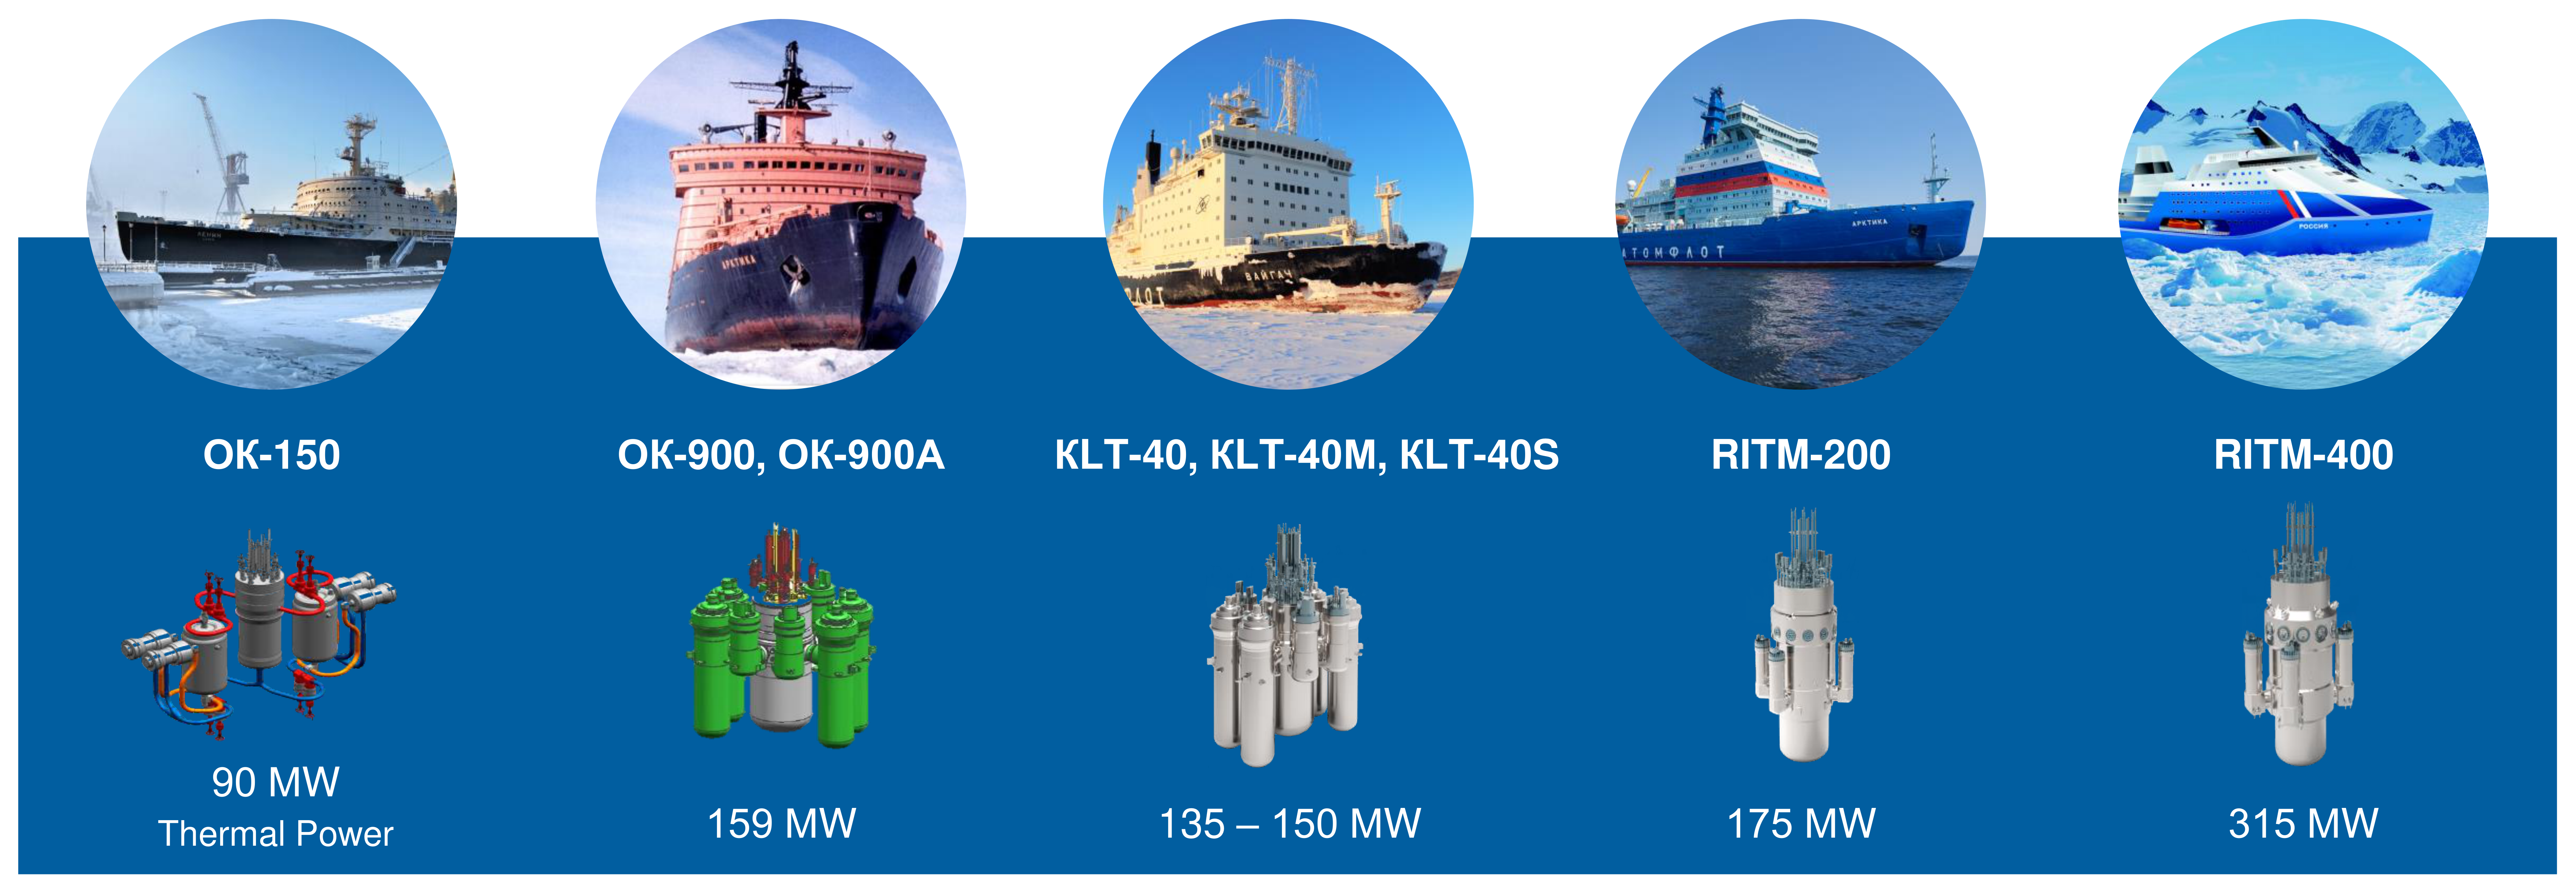
\includegraphics[width=\textwidth]{images/lr_okbm_icebreaker_reactors.png}
  \caption[Afrikantov OKBM reactors for nuclear icebreakers]{Afrikantov OKBM reactors for nuclear icebreakers.\newline Figure taken from~\cite{rosatom_presentation}.}
  \label{fig:lr-okbm-reactors}
\end{figure}

Two members of this line are documented in sufficient detail to be
useful here:

\begin{itemize}
  \item The KLT-40S is deployed in the floating nuclear power plant
        (FNPP) \emph{Akademik Lomonosov}. It uses uranium dioxide
        (UO$_2$) dispersed in a silumin matrix at 18.6~wt\% uranium-235,
        a core of 121 fuel assemblies, and a refuelling cycle of 30 to
        36 months~\cite{worldnuclearreport_smr}.

  \item The RITM-200N, the land-based member of the family, is rated
        190~MWth and 55~MWe gross and uses uranium enriched below
        20~wt\%~\cite{ritm200n_nei_2024}.
\end{itemize}

The relevance of the RITM-200N to this work is that its designers
describe its fuel cassettes as analogues of those used in the cores of
the RITM-200 and KLT-40S icebreakers~\cite{ritm200n_nei_2024}. The
transfer of a marine core to a land-based prototype is therefore
established practice, and the Brazilian programme follows it.

\subsubsection{The French lineage}
\label{subsec:lineage-france}
The K15 is an integral pressurised water reactor of 150~MWth. It and
its successor are used as follows~\cite{wna_ships}:

\begin{itemize}
  \item Two K15 units power the aircraft carrier \emph{Charles de
        Gaulle}, which runs five years between refuellings.

  \item The Le~Triomphant ballistic missile submarines use the same
        reactor.

  \item The Barracuda submarines carry 150~MWth reactors based on the
        K15, with a refuelling interval of about ten
        years~\cite{wna_ships}.
\end{itemize}

Newer French naval reactors run
on low-enriched uranium (LEU), at 7.5~wt\% in the Caramel fuel and about
5 to 6~wt\% in the Barracuda class~\cite{wna_ships}. The French line is the closest Western analogue to the present work.
Its naval propulsion cores operate below the 20~wt\% threshold that
separates LEU from highly enriched uranium (HEU)~\cite{nrc_10cfr110_2}.

\subsubsection{The United States and United Kingdom lineage}
\label{subsec:lineage-us-uk}
Naval reactors of the United States and the United Kingdom use
weapon-grade HEU. The enrichment is 93 to 97~wt\% uranium-235 in current
United States practice~\cite{jason_2016}, and it was 97.3~wt\% in United
States and British submarines in 1990~\cite{ippolito_1990}.

The feasibility of converting these cores to LEU at 19.75~wt\% has been
examined in two open assessments:

\begin{itemize}
  \item The report of the JASON advisory panel assessed the low-enriched
        fuel concept proposed by the Naval Nuclear Propulsion Program and
        the plan to develop and qualify it~\cite{jason_2016}.

  \item The report of the Office of Naval Reactors to Congress set out a
        conceptual research and development plan for a low-enriched naval
        fuel~\cite{onr_leu_2016}.
\end{itemize}

The second report assumes LEU at 19.75~wt\%, the highest enrichment
within the internationally recognised definition of
LEU~\cite{onr_leu_2016}. This work adopts 19.75~wt\% as the upper bound
of the enrichment range at the start of the optimisation study of the
core.

\subsubsection{The Brazilian lineage}
\label{subsec:lineage-brazil}
The Programa Nuclear da Marinha of the Brazilian Navy began in
1979~\cite{vasconcelos_fapesp_2025}. It is divided into two main
undertakings~\cite{marinha_relatorio_gestao_2025}:

\begin{itemize}
  \item The development of nuclear technology in the area of reactors.

  \item The mastery of the nuclear fuel cycle.
\end{itemize}

These two undertakings support the development and operation of the
land-based prototype of an embarked nuclear plant and of the plant of
the nuclear-powered submarine itself~\cite{marinha_relatorio_gestao_2025}.
That prototype is LABGENE, the Laboratório de Geração de Energia
Nucleoelétrica~\cite{marinha_relatorio_gestao_2025}. It is the
land-based prototype for the reactor of the submarine Álvaro
Alberto~\cite{vasconcelos_fapesp_2025} and is located at the Centro
Industrial Nuclear de Aramar (Cina) in Iperó, São
Paulo~\cite{ctmsp_visita_2018,vasconcelos_fapesp_2025}.

Figure~\ref{fig:vessel-components} identifies the components of a
pressurised water reactor vessel on the envelope adopted for the
LABGENE-class model. The envelope follows the simplified vessel drawing
prepared for a structural analysis according to the Centro
Tecnológico da Marinha em São Paulo (CTMSP)~\cite{maruyama_2013}.

The internals, the coolant path and the control rods in the figure are
illustrative and are not to scale. The coolant enters at the inlet
nozzle, descends the downcomer, passes through the lower plenum and the
core, and leaves at the outlet nozzle.

\begin{figure}[htbp]
  \centering
  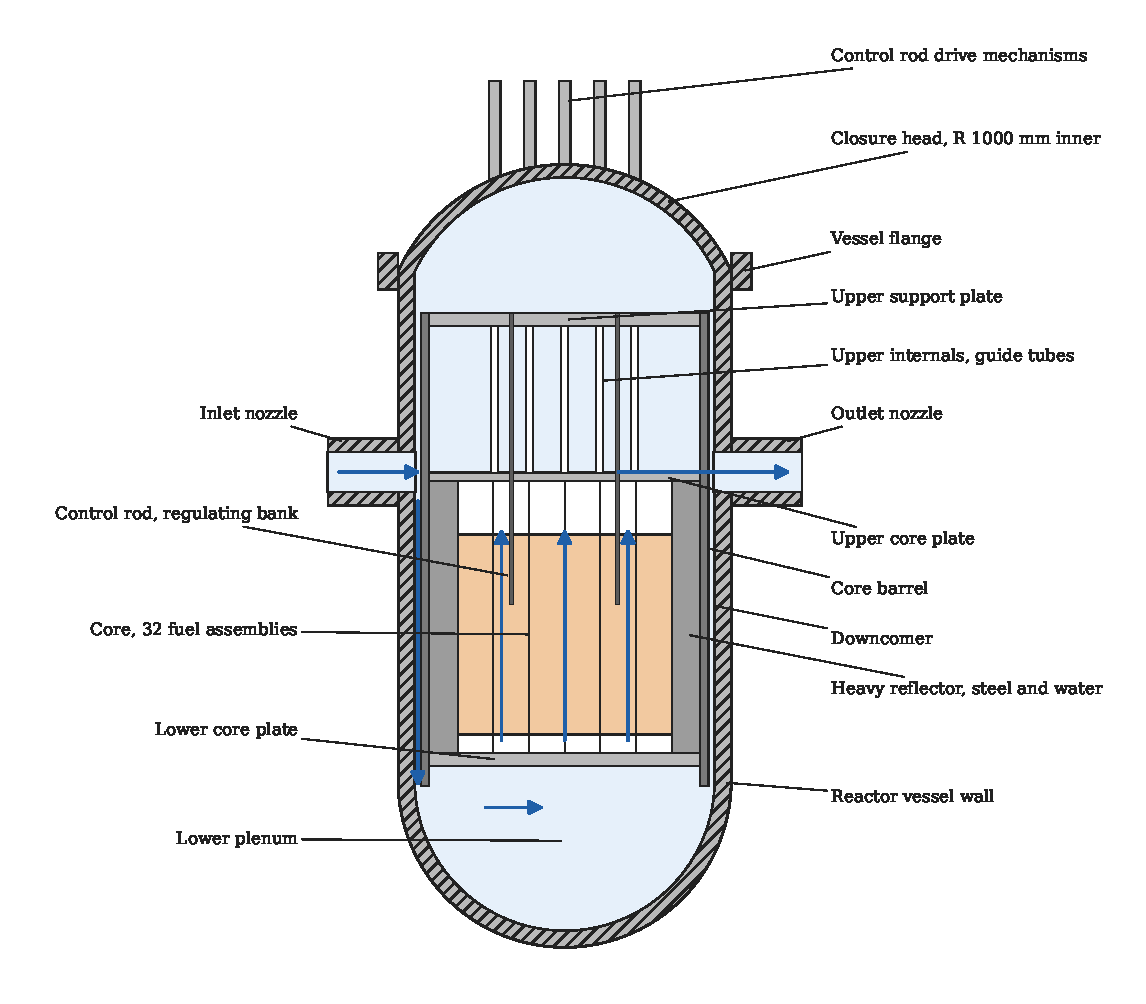
\includegraphics[width=0.95\textwidth]{images/th_vessel_components}
  \caption[Components of a pressurised water reactor vessel]{Components of a pressurised water reactor vessel, drawn on the LABGENE-class vessel envelope.\newline Vessel envelope adapted from~\cite{maruyama_2013}.}
  \label{fig:vessel-components}
\end{figure}

The open record establishes the following facts about the LABGENE
plant:

\begin{itemize}
  \item It is a pressurised water reactor with primary, secondary and
        cooling circuits, developed by the Navy for the submarine and
        tested first on land~\cite{ctmsp_labgene_2015}.

  \item According to the Navy, as reported by the specialised press, the
        reactor generates 48~MW of thermal
        power~\cite{demartini_nuclep_2022}, equivalent to 11~MWe for the
        prototype~\cite{galante_podernaval_2020}. The academic literature
        gives 48 to 50~MWth for the submarine
        reactor~\cite{dinizcosta_2017}.

  \item Its fuel is low-enriched uranium, as declared by Brazil at the
        2026 Review Conference of the Non-Proliferation
        Treaty~\cite{brazil_npt_wp13_2026}. The fuel consists of UO$_2$
        pellets in rods grouped into fuel
        elements~\cite{marinha_inb_labgene_2022,pereira_rmb_2023}.
        Ind\'ustrias Nucleares do Brasil (INB) produced the pellets of
        the LABGENE fuel between August and December
        2021~\cite{marinha_inb_labgene_2022}.

  \item The submarine will be a nuclear-powered, conventionally armed
        vessel. The land-based prototype reactor, the submarine, its
        reactor and its fuel are designed and built in
        Brazil~\cite{brazil_npt_wp13_2026}.

  \item The submarine is named \'Alvaro Alberto and is part of the
        Programa de Desenvolvimento de Submarinos (PROSUB), a partnership
        between Brazil and France~\cite{vasconcelos_fapesp_2025}.
\end{itemize}

The enrichment of the LABGENE fuel is reported inconsistently in open
sources:

\begin{itemize}
  \item In 2014 the chairman of the Navy's nuclear-propelled submarine
        development programme told the Foreign Relations and National
        Defence Committee of the Federal Senate that the fuel would be
        enriched to 6 to 8~wt\%~\cite{dinizcosta_2017}.

  \item Kassenova reported 18 to 19~wt\%~\cite{kassenova_2014}, a figure
        given by a former chairman of the Comiss\~ao Nacional de Energia
        Nuclear in 2005~\cite{dinizcosta_2017}.

  \item In 2025 Pesquisa FAPESP reported from Aramar that the submarine
        fuel enrichment will reach 19~wt\%. It quoted the director of
        CTMSP stating that the first fuel load had already been
        produced~\cite{vasconcelos_fapesp_2025}.
\end{itemize}

The refuelling interval is given as five years~\cite{dinizcosta_2017},
but no lattice pitch, assembly count, burnable poison loading, soluble
boron concentration or peaking factor for the LABGENE core is available
from any open source. The only open geometric information is the simplified
vessel drawing published in a structural dissertation carried out for
CTMSP. It gives the following dimensions~\cite{maruyama_2013}, shown in
Figure~\ref{fig:lr-maruyama-vessel}:

\begin{itemize}
  \item A cylindrical inner radius of 900~mm.

  \item A wall thickness of 100~mm.

  \item An overall height of 4700~mm.
\end{itemize}

\begin{figure}[htbp]
  \centering
  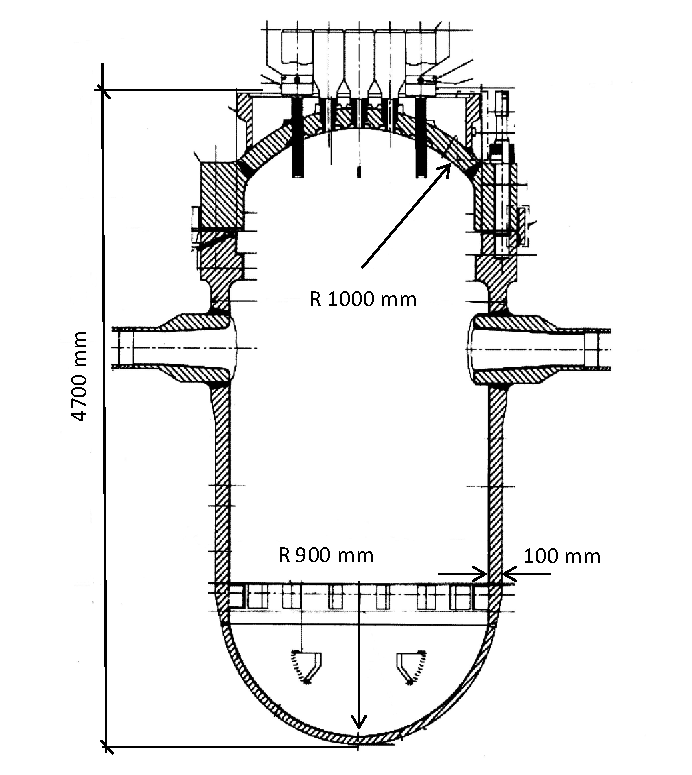
\includegraphics[width=0.55\textwidth]{images/lr_maruyama_vessel.pdf}
  \caption[Vessel dimensions adopted according to CTMSP]{Reactor vessel dimensions adopted according to CTMSP.\newline Figure taken from~\cite{maruyama_2013}.}
  \label{fig:lr-maruyama-vessel}
\end{figure}

Because the core data are closed, the present work is framed as a study
of a LABGENE-class core. Four inputs are taken from the open record:

\begin{itemize}
  \item The rated power.

  \item The PWR architecture.

  \item The low-enriched fuel.

  \item The vessel envelope.
\end{itemize}

Every remaining core parameter is an independent modelling choice of
this thesis and carries no claim of correspondence with the actual
prototype. These parameters are the following:

\begin{itemize}
  \item The enrichment zoning.

  \item The lattice pitch.

  \item The assembly count.

  \item The gadolinia (Gd$_2$O$_3$) loading.

  \item The poisoned-pin count.

  \item The reflector thickness.
\end{itemize}

The enrichment range at the start of the study, 2.0 to 19.75~wt\%, was
set from the open information and encloses the whole range reported for
the prototype. The
final campaign, constrained by the controllability screen of
Section~\ref{sec:meth-ctrl}, admits assembly enrichments up to
13.9~wt\%. The 19~wt\% reported for the prototype therefore lies inside
the explored range but outside the final candidate space.

\subsection{Open academic analyses}
\label{subsec:naval-academic}

Two bodies of open academic work give design data for compact
low-enriched cores. This thesis uses them for two questions: how
enrichment, core size and core life trade against each other, and how
far the power density and peaking of a boron-free marine core can go.

\subsubsection{Ippolito's comparison of submarine cores}
\label{subsec:academic-ippolito}

The thesis of Ippolito asked what a submarine core loses, in size and
in life, when its fuel changes from highly enriched to low-enriched
uranium~\cite{ippolito_1990}. Three cores of the same thermal power,
50~MWth, were designed to answer it. That power is close to the
48~MWth of the LABGENE-class core.

The three cores differ in the enrichment and in the form of their fuel.
Table~\ref{tab:lr-ippolito} shows what each one achieves.

\begin{table}[!htbp]
  \centering
  \caption{Submarine cores of 50~MWth compared by Ippolito: fuel, size and core life.}
  \label{tab:lr-ippolito}
  \small
  \begin{tabular}{@{}cccc@{}}
    \toprule
    Enrichment & Fuel & Core volume & Core life \\
    (wt\% $^{235}$U) & & (L) & (full-power days) \\
    \midrule
    7    & UO$_2$, caramel   & 506 & 600  \\
    20   & UO$_2$, caramel   & 667 & 1200 \\
    97.3 & UO$_2$/Zr cermet  & 265 & 1200 \\
    \bottomrule
  \end{tabular}

  \vspace{2pt}
  {\footnotesize Data from~\cite{ippolito_1990}.}
\end{table}
\FloatBarrier

The table reads as follows~\cite{ippolito_1990}:

\begin{itemize}
  \item \textbf{Same life, larger core:} the 20~wt\% core lasts as long as
        the 97.3~wt\% core, 1200 full-power days, which is about 3.3
        years at full power. It needs about two and a half times the
        volume, 667~L against 265~L.

  \item \textbf{Lower enrichment, shorter life:} the 7~wt\% core cannot
        stay critical for 1200 full-power days and lasts 600.

  \item \textbf{A manageable size penalty:} the 20~wt\% core is 24~cm wider
        and 30~cm taller than the 97.3~wt\% core. Ippolito judged that an
        integral reactor, with the steam generators inside the pressure
        vessel, can compensate for that increase.
\end{itemize}

The study also shows that the placement of the gadolinia changes its
effect~\cite{ippolito_1990}:

\begin{itemize}
  \item Mixed uniformly into the fuel, gadolinia reduced the reactivity
        to be controlled at the beginning of the cycle, but it burned out
        quickly because nothing shielded it from the neutrons.

  \item Concentrated in separate plates, gadolinia gave a peak of excess
        reactivity near the end of the cycle.
\end{itemize}

This thesis takes two points from the study. A 50~MWth core on
low-enriched uranium can last several years, at the price of a larger
core. The way the gadolinia is distributed in the fuel decides how its
hold-down changes through the cycle.

\subsubsection{The Cambridge studies of civil marine cores}
\label{subsec:academic-cambridge}

The Cambridge studies designed a soluble-boron-free PWR core for civil
marine propulsion with a life of 15 effective full-power years and fuel
below 20\%~$^{235}$U. Two of them are used here, in support of the
long-life, boron-free and heavily poisoned design logic of
Section~\ref{subsec:comparison} and of the power density entries of
Table~\ref{tab:naval-vs-commercial}:

\begin{itemize}
  \item The first part of the core design study works at assembly
        level, on the fissile loading, the burnable poisons and the
        control rods~\cite{alam_partI_2019}. The high fissile loading
        needed for the long life makes the beginning-of-life reactivity
        very high. A self-shielded burnable absorber keeps the assembly
        reactivity low and stable with relatively little burnup
        penalty~\cite{alam_partI_2019}.

  \item The hot channel analysis coupled neutronics and thermal
        hydraulics for a 375~MWth version of the core, with 16\% UO$_2$
        and 19.25\% duplex fuel~\cite{alam_2019_hotchannel}. The average
        power density of the reference core, about 63~MW/m$^3$, could
        be raised to 100~MW/m$^3$ while every thermal-hydraulic limit was
        met. At 111~MW/m$^3$ the surface heat flux, the fuel temperature
        and the pressure drop exceeded their limits. Power peaking stayed
        below the industry limit of 1.5, and the minimum departure from
        nucleate boiling ratio was not the limiting
        factor~\cite{alam_2019_hotchannel}.
\end{itemize}

\subsection{Comparison of naval-heritage and commercial small modular PWR cores}
\label{subsec:comparison}

Table~\ref{tab:naval-vs-commercial} contrasts the two design families on
the characteristics most relevant to core and fuel design. Every entry
is traceable to a named open source. The detailed criteria of classified
naval programmes are not verifiable in open sources.

\begin{table}[htbp]
  \centering
  \footnotesize
  \caption{Naval-heritage and commercial small modular PWR cores: design characteristics.}
  \label{tab:naval-vs-commercial}
  \begin{tabularx}{\textwidth}{@{}>{\raggedright\arraybackslash}p{2.8cm} >{\raggedright\arraybackslash}X >{\raggedright\arraybackslash}X@{}}
    \toprule
    \textbf{Characteristic} & \textbf{Naval-heritage core} &
    \textbf{Commercial SMR core} \\
    \midrule
    Fuel enrichment &
    HEU of 93 to 97~wt\% in US and UK practice~\cite{jason_2016}, and LEU
    below 10~wt\% in French submarines~\cite{ippolito_1990}. 18.6~wt\% in
    the KLT-40S~\cite{worldnuclearreport_smr} &
    LEU below 5~wt\%~\cite{iaea_smr_2024}, up to 4.95~wt\% in the NuScale
    fuel design~\cite{nuscale_htp2_2017} \\
    \addlinespace
    Refuelling interval &
    30 to 36 months for the KLT-40S~\cite{worldnuclearreport_smr}. Five
    years for the \emph{Charles de Gaulle} and about ten years for the
    K15-based Barracuda reactors~\cite{wna_ships} &
    18 to 24 months~\cite{iaea_smr_2024} \\
    \addlinespace
    Soluble boron &
    Soluble-boron-free operation proposed for civil marine
    cores~\cite{alam_partI_2019} &
    Borated coolant, with boron-free variants such as the ACP100 and the
    i-SMR~\cite{acp100_physor2020,ismr_sbf_2024} \\
    \addlinespace
    Burnable poison &
    A major share of the hold-down of a high beginning-of-life
    reactivity~\cite{alam_partI_2019,ippolito_1990} &
    Gd$_2$O$_3$ up to 8~wt\% in the NuScale fuel
    design~\cite{nuscale_htp2_2017} \\
    \addlinespace
    Power density &
    Up to about 100~MW/m$^3$~\cite{alam_2019_hotchannel} &
    60 to 65~MW/m$^3$~\cite{alam_2019_hotchannel} \\
    \addlinespace
    Motion and shock &
    Qualified for inclination, motion and shock~\cite{ritm200n_nei_2024} &
    Land-based siting~\cite{iaea_smr_2024} \\
    \addlinespace
    Reactivity control &
    Control rods with compensating groups~\cite{worldnuclearreport_smr} &
    Control rods plus soluble boron, or rods plus burnable poison in
    boron-free designs~\cite{acp100_physor2020,ismr_sbf_2024} \\
    \bottomrule
  \end{tabularx}
\end{table}

The differences collected in Table~\ref{tab:naval-vs-commercial} follow
from a small set of naval operational requirements. Each requirement
has a consequence for the core:

\begin{enumerate}
  \item Energy autonomy without frequent refuelling asks for a compact
        core with a large energy reserve, which higher enrichment
        provides~\cite{ippolito_1990}.

  \item High availability at sea asks for long refuelling intervals. The
        fissile loading needed for a long life gives a high
        beginning-of-life reactivity~\cite{alam_partI_2019}.

  \item Soluble-boron-free operation simplifies the plant and saves
        space. It removes the corrosive effect of the boron, improves the
        moderator temperature coefficient and eliminates boron dilution
        accidents, including dilution by seawater if the ship
        sinks~\cite{alam_partI_2019}.

  \item Heavy reliance on movable rods is avoided, so the burnable poison
        carries a major part of the reactivity control. A self-shielded
        absorber keeps the assembly reactivity low and stable with little
        burnup penalty~\cite{alam_partI_2019}.

  \item Compactness within the hull raises the volumetric power density
        and tightens the margin to the hot channel limit expressed by
        $F_{\Delta H}$~\cite{alam_2019_hotchannel}.

  \item A ship must also vary its power easily~\cite{alam_partI_2019},
        which in a boron-free core falls to the regulating rods.

  \item Qualification for inclination, motion and shock adds structural
        and thermal-hydraulic margins~\cite{ritm200n_nei_2024}. It is
        recorded in the table for completeness and is not acted on in
        this work, whose model carries no thermal-hydraulic feedback.
\end{enumerate}

Four of these requirements enter the design space and the objectives of
this thesis:

\begin{itemize}
  \item The enrichment.

  \item The burnable poison inventory.

  \item The boron strategy.

  \item The power density.
\end{itemize}

\subsection{Positioning of the LABGENE-class 48\texorpdfstring{\,}{ }MWth core}
\label{subsec:positioning}

The core studied in this thesis is a LABGENE-class 48~MWth pressurised
water reactor of naval heritage. Among designs with open documentation,
the closest operating analogues are the KLT-40S and the RITM-200 family.
They share the naval logic of a compact low-enriched-uranium core with a
long refuelling
interval~\cite{worldnuclearreport_smr,ritm200n_nei_2024}.

The core would drive the land-based propulsion prototype at LABGENE,
whose visual mock-up is shown in Figure~\ref{fig:lr-labgene-blocks}.
The plant is arranged in three blocks, listed below from the reactor
outwards~\cite{galante_podernaval_2020b}:

\begin{itemize}
  \item Block 40 holds the primary circuit: the reactor pressure vessel,
        the steam generators, the pressuriser and the primary pumps.

  \item Block 30 holds the secondary circuit: the turbogenerators with
        their lubrication system, the condenser and the steam generator
        feedwater pumps.

  \item Block 20 holds the propulsion line: the electric propulsion
        motor, the speed-increasing gearbox and the dynamometer brake that
        absorbs the shaft power in place of a propeller.
\end{itemize}

\begin{figure}[htbp]
  \centering
  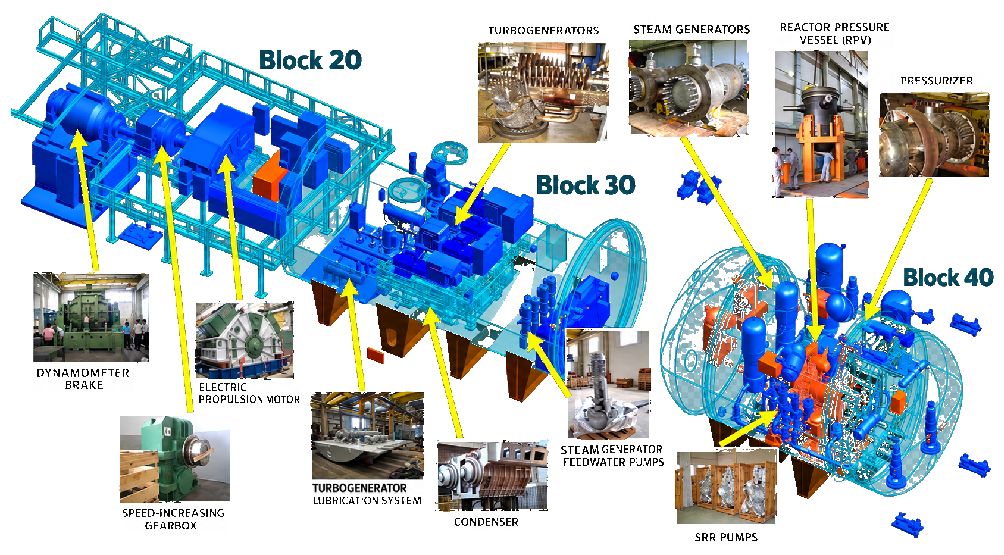
\includegraphics[width=\textwidth]{images/lr_labgene_blocks.pdf}
  \caption[Mock-up of the LABGENE land-based prototype]{Visual mock-up of the LABGENE land-based prototype.\newline Figure adapted from~\cite{galante_podernaval_2020b}.}
  \label{fig:lr-labgene-blocks}
\end{figure}

The optimisation objectives map directly onto the naval requirements:

\begin{itemize}
  \item The cycle length maps onto the requirement of long core life.

  \item The radial enthalpy-rise hot channel factor $F_{\Delta H}$ maps
        onto compact high-power-density operation.
\end{itemize}

The design variables are the levers of a long-life core, namely the
fissile loading, the burnable absorber and the geometry of the lattice
and of the reflector. The soluble boron is held constant at the
1000~ppm of the NuScale-like benchmark from which the assembly geometry
is taken, and the constraint on the beginning-of-life multiplication
factor is applied with that boron present
(Section~\ref{sec:meth-boron}). The design variables are the following:

\begin{itemize}
  \item The enrichment.

  \item The gadolinia concentration and the poisoned-pin count.

  \item The pin pitch.

  \item The reflector thickness.
\end{itemize}

The enrichment range explored in Campaigns 1 to 6, 2.0 to 19.75~wt\%,
encloses every figure reported for the prototype. Those figures range
from the 6 to 8~wt\% stated in 2014~\cite{dinizcosta_2017} to the
19~wt\% reported in 2025~\cite{vasconcelos_fapesp_2025}, so the
optimisation does not presuppose any of them.

The controllability screen of the final campaign then bounds the
candidate space at 13.9~wt\%, below the highest reported figure. That
bound is itself a result on the prototype envelope.

\section{Optimisation of nuclear reactor cores: development and state
of the art}
\label{sec:lit-opt}

Section~\ref{sec:smr-naval} fixed the design envelope of the core
studied here: its thermal power, its fuel class, the vessel that bounds
it and the refuelling interval it has to meet. Those quantities enter
the present work as fixed input data and as constraints on the design
space. This section reviews the methods by which a core is optimised
within such an envelope.

Fuel reloading and core design optimisation keep the cycle length, the
power level and the feedback within their targets by choosing the
following quantities~\cite{stewart_2021}:

\begin{itemize}
  \item The arrangement of the assemblies.

  \item The core geometry.

  \item The material composition.
\end{itemize}

The field has six decades of history, and its methods track the wider
history of engineering optimisation. The review proceeds in three
parts:

\begin{enumerate}
  \item The chronological development of the methods, from mathematical
        programming to machine learning
        (Sections~\ref{sec:lit-opt-early} to
        \ref{sec:lit-opt-surrogate}).

  \item The structural difficulties of the field, above all the
        difficulty introduced by burnup
        (Sections~\ref{sec:lit-opt-difficulties}
        and \ref{sec:lit-opt-burnup}).

  \item The current state of the art, with the strengths and
        limitations of each family of methods and the positioning of
        the present work (Section~\ref{sec:lit-opt-sota}).
\end{enumerate}

\subsection{Mathematical programming and the Haling principle}
\label{sec:lit-opt-early}

Mathematical programming was applied to in-core fuel management in
three forms:

\begin{itemize}
  \item Dynamic programming, in the work of Wall and Fenech in
        1965~\cite{meneses_2010}.

  \item Linear and quadratic programming, in the work of Tabak in
        1968~\cite{meneses_2010}.

  \item Linear programming for the refuelling schemes of light water
        reactors, and optimal control for the time-dependent management
        of the control poison~\cite{downar_1988}.
\end{itemize}

The most influential idea of the era is the Haling principle. If the
power in each region is held constant through the cycle, the depletion
follows a straight line in reactivity space and the power peaking can be
no higher or lower at any point of the cycle. That constant shape gives
the minimum peaking, and the end-of-cycle state follows from a single
depletion~\cite{downar_1988}.

The principle became the standard shortcut of the period because it
removed the need to march every candidate design through time. Its use
rests on the assumption that the Haling power distribution closely
resembles the power shape of the final, detailed core
design~\cite{downar_1988}.

The deterministic era carried a structural weakness. Linear programming
uses only first derivatives of the objective and cannot distinguish a
local from a global optimum, so different starting points can return
different solutions~\cite{downar_1988}. This is a serious limitation in
a design space that is discrete, nonconvex and rich in local optima.

\subsection{Heuristics, knowledge-based systems and perturbation
theory}
\label{sec:lit-opt-heuristic}

The 1980s produced two complementary responses to that mismatch. The
first automated the search itself. Hobson and Turinsky determined
the loading pattern that maximises beginning-of-cycle reactivity under
power peaking and discharge burnup constraints. Their method combined
two tools~\cite{hobson_turinsky_1986}:

\begin{itemize}
  \item Monte Carlo integer programming as the search.

  \item First-order perturbation theory to estimate the effect of each
        assembly shuffle.
\end{itemize}

Designer knowledge was also encoded directly. Logical rules for
generating loading patterns appear as early as 1972, and expert systems
became one of three kinds of decision-support
tool~\cite{meneses_2010}:

\begin{itemize}
  \item Manual design packages.

  \item Optimisation packages.

  \item Expert systems.
\end{itemize}

The second response was generalised perturbation theory (GPT). GPT
estimates how the core eigenvalue and the power distribution respond to
a fuel shuffle without a full re-solution of the transport problem. It
was demonstrated for three-dimensional design optimisation of Canada
Deuterium Uranium (CANDU) reactors~\cite{rozon_beaudet_1992}.

GPT then became the neutronics engine of the FORMOSA-P code. There a
nodal GPT model evaluates objectives and constraints cheaply enough to
sit inside a stochastic search, and the method was extended even to the
feed enrichment as a decision variable~\cite{maldonado_1995}. That model
is of higher order, because first-order perturbation techniques proved
inadequate for loading pattern changes~\cite{maldonado_1995}.

Perturbation methods have known limits:

\begin{itemize}
  \item First-order perturbation theory is accurate only for small
        changes from the reference state~\cite{hobson_turinsky_1986}.

  \item Depletion perturbation theory cannot accurately represent
        assembly movement or the strong flux perturbations introduced
        by burnable absorbers~\cite{downar_1988}.
\end{itemize}

\subsection{Stochastic global search}
\label{sec:lit-opt-stochastic}

At the turn of the 1990s, the field accepted that the design space is
nonconvex and moved to stochastic global search. Kropaczek and Turinsky combined simulated annealing with a core physics
model based on second-order generalised perturbation theory for PWR
reload design. Their code places the feed fuel, the burnt fuel with its
orientation and the burnable poisons to reach one of three objectives,
with the limits on peaking, burnup and moderator temperature coefficient
enforced either by penalty functions or by rejecting the exchanges that
violate them~\cite{kropaczek_turinsky_1991}:

\begin{itemize}
  \item Maximise the multiplication factor at a target end-of-cycle
        burnup.

  \item Minimise the maximum radial power peaking over the cycle.

  \item Maximise the discharge burnup.
\end{itemize}

Genetic algorithms, which evolve a population of candidate solutions by
mimicking natural selection~\cite{deb_2001}, entered the field shortly
after. Poon and Parks applied them to the positions and orientations of
the fuel assemblies together with their burnable poison, and tabu search
was applied with similar success~\cite{meneses_2010}.

At the end of the decade, Yamamoto compared these heuristics on equal
terms. A single benchmark, the loading pattern of a Westinghouse
three-loop PWR of 900~MWe with 157 assemblies, was solved ten times with
each method, with the aim of maximising the cycle length while keeping
the radial peaking factor below 1.435. The comparison gave the following
results~\cite{yamamoto_1997}:

\begin{itemize}
  \item Direct search and binary exchange evaluated the fewest loading
        patterns, but they were trapped in local optima and reached the
        lowest quality.

  \item Simulated annealing and the genetic algorithm reached better
        patterns. The slowest cooling schedule of simulated annealing
        needed about 10\,300 evaluated patterns on average, against 3000
        for the genetic algorithm.

  \item A hybrid of the genetic algorithm with binary exchange performed
        best, because the global search of the first and the local search
        of the second compensated for each other's weaknesses.
\end{itemize}

For the present work, the most relevant result of the period is the
first nondominated genetic search for PWR reload
design~\cite{parks_1996}. Parks applied it to the reload core of a
Westinghouse three-loop PWR, with three objectives optimised at the same
time~\cite{parks_1996}:

\begin{itemize}
  \item Minimise the feed enrichment.

  \item Maximise the discharge burnup.

  \item Minimise the radial form factor.
\end{itemize}

The usual alternative adds the objectives into one weighted function.
Each run then returns a single design, whose position on the trade-off
depends on the weights the designer chose, so the trade-off can only be
explored with many runs~\cite{parks_1996}.

The nondominated search ranks the designs of its population by Pareto
dominance and keeps an archive of the designs that no other design beats
in every objective. One run therefore returns the whole trade-off
surface, and the designer picks from it the designs worth closer
study~\cite{parks_1996}.

This is the Pareto-based formulation that the Non-dominated Sorting
Genetic Algorithm II (NSGA-II) later standardised~\cite{deb_nsga2_2002}.
\textbf{This thesis adopts it}, so its result is a Pareto front of possible core
designs and the choice among them is left to the designer.

\subsection{Population-based metaheuristics and multi-objective
evolutionary algorithms}
\label{sec:lit-opt-population}

The 2000s and 2010s widened the toolbox with swarm algorithms. The survey
of Stewart, Palmer and DuPont reports three examples~\cite{stewart_2021}:

\begin{itemize}
  \item Yadav and Gupta (2011) applied particle swarm optimisation to
        find PWR core configurations with reasonably low peaking factors,
        using a conventional neutron transport solver and no surrogate
        model.

  \item Safarzadeh et al.\ (2014) used a hybrid bee colony algorithm to
        reduce the time needed to find reload patterns for the core of a
        VVER-1000 pressurised water reactor, in comparison with a standard
        particle swarm optimisation.

  \item Domingos, Schirru and Pereira (2006) found particle swarm
        optimisation easier to model than evolutionary methods, and less
        costly for the same results on simplified core geometries.
\end{itemize}

Brazilian researchers of the COPPE/UFRJ group, at the Federal University
of Rio de Janeiro, worked on the reload optimisation problem of Angra~1,
a Westinghouse pressurised water reactor in commercial operation at Angra
dos Reis, Brazil, since 1985~\cite{eletronuclear_angra1}. At each
refuelling, part of the fuel is replaced, and the assemblies are
rearranged, and the group used the seventh operating cycle of the plant
as a common test case for choosing that arrangement. Four methods were
applied to it and compared~\cite{meneses_2010}:

\begin{itemize}
  \item The Ant-Q ant colony algorithm.

  \item Artificial ant colony connective networks.

  \item Population-based incremental learning.

  \item Particle swarm optimisation with random keys.
\end{itemize}

On the multi-objective side, NSGA-II~\cite{deb_nsga2_2002} and SPEA are
the two multi-objective genetic algorithms most widely used in
research~\cite{stewart_2021}. They rest on the broader theory of
multi-objective evolutionary algorithms
(MOEAs)~\cite{deb_2001,coello_2007}.

An MOEA is a population-based search that applies the evolutionary
operators of selection, crossover and mutation to a set of candidate
designs. Because it processes a whole population at every iteration, its
outcome is also a population, and it can find several Pareto-optimal
solutions in one run without first merging the objectives into a single
function~\cite{deb_2001}. Such an algorithm pursues two goals at the same
time~\cite{deb_2001}:

\begin{itemize}
  \item Convergence, meaning a set of solutions as close as possible to
        the Pareto-optimal front.

  \item Diversity, meaning a set of solutions spread as widely as
        possible along that front.
\end{itemize}

In his book on multi-objective optimisation with evolutionary algorithms,
Deb (2001) classifies MOEAs by whether they preserve elitism, that is, whether
the best solutions of a population are carried directly into the next
generation. VEGA, MOGA, NSGA and NPGA are non-elitist algorithms, while
NSGA-II, SPEA and PAES preserve the elite~\cite{deb_2001}.

\subsection{Surrogate-assisted optimisation and machine learning}
\label{sec:lit-opt-surrogate}

The binding constraint of every method above is the number of calls to
the expensive simulator. Surrogate-assisted evolutionary computation
addresses it directly, in three steps~\cite{jin_2011}:

\begin{enumerate}
  \item A cheap statistical model is trained on evaluated designs.

  \item The optimiser searches the model.

  \item The simulator is reserved for the most informative candidates.
\end{enumerate}

Gaussian process regression is the canonical surrogate. Its prediction
carries an uncertainty that is reduced close to the evaluated designs
and grows away from them~\cite{rasmussen_gp_2006}.

The Gaussian process, known in engineering design as Kriging, suits
problems in which every sample comes from an expensive simulation. Such
samples must be used sparingly, and their number is often small because
each one carries a computational cost~\cite{forrester_book_2008}. Two
properties make the model a good choice in this setting:

\begin{itemize}
  \item It estimates its own error. The predictive variance shows where
        the model is uncertain, so new samples can be placed where they
        improve it most, which Forrester, Sobester and Keane call a key
        advantage of Gaussian process models~\cite{forrester_book_2008}.
        The Gaussian process is also the surrogate most often used to
        estimate model uncertainty in evolutionary
        optimisation~\cite{jin_2011}.

  \item Its cost is affordable for a modest data set. Exact Gaussian
        process prediction scales as $\mathcal{O}(n^3)$ with the number
        $n$ of training points, which becomes prohibitive for large data
        sets~\cite{rasmussen_gp_2006}. The guideline of Forrester,
        Sobester and Keane places Kriging models within reach for fewer
        than about 20 variables and 500 samples, and points to support
        vector regression, fixed radial basis functions or polynomials
        beyond that range~\cite{forrester_book_2008}.
\end{itemize}

The problem of this thesis falls inside that range. It has four to six
design variables, and each completed campaign evaluated between 36 and
114 designs, each one a Monte Carlo depletion. \textbf{For these reasons, a
Gaussian process was chosen as the surrogate model of this thesis.}

The loop is initialised by a space-filling sampling plan, which spreads
the first designs over the design space before any surrogate exists.
McKay, Beckman and Conover compared three ways of choosing these
inputs~\cite{mckay_lhs_1979}:

\begin{enumerate}
  \item Random sampling, in which the input vectors are drawn at random
        from their joint distribution.

  \item Stratified sampling, in which the sample space is divided into
        disjoint strata and a random sample is drawn from each stratum,
        so that every region of the space is represented.

  \item Latin hypercube sampling, in which the range of each variable is
        divided into $N$ intervals of equal probability, one value is
        drawn from each interval, and the values of the different
        variables are matched at random.
\end{enumerate}

In their comparison, Latin hypercube sampling estimated the mean, the
variance, and the distribution function of the output with a smaller
spread than the other two methods. It improves on random sampling when
certain monotonicity conditions hold~\cite{mckay_lhs_1979}.

After the initial plan, the loop is driven by infill criteria that
balance exploration against exploitation. A criterion such as the
expected improvement weighs the prediction of the surrogate against its
uncertainty, so new designs are placed both where the prediction is
promising and where the model knows least~\cite{forrester_book_2008}.

For multi-objective problems, the hypervolume indicator, the volume of
objective space weakly dominated by a front, measures the quality of
that front~\cite{zitzler_2003_performance}. It can also serve as the
target of the infill selection.

Surrogate-assisted search is the first of two recent frontiers in
nuclear core optimisation, and its applications are growing:

\begin{enumerate}
  \item Deep neural network surrogates coupled to NSGA-II for the loading
        patterns of a 36-assembly microcore, a 37-assembly small modular
        core and a 193-assembly PWR core~\cite{whyte_2020}.

  \item A convolutional neural network surrogate combined with a
        genetic algorithm for reload pattern
        optimisation~\cite{wan_2022}.

  \item Neural network acceleration of a genetic algorithm for a
        coupled fast and thermal experiment whose design space exceeds
        $3\times10^{71}$ configurations~\cite{pevey_2022}.
\end{enumerate}

Deep reinforcement learning is the second frontier, after the
surrogate-assisted search described above. The results below are
reported by the developing groups, and independent replication remains
limited:

\begin{itemize}
  \item Physics-informed reinforcement learning for assembly design is
        reported by its authors to find several times more feasible
        patterns than stochastic optimisation at a markedly lower
        computational cost~\cite{radaideh_2021_rl}.

  \item The NEORL framework packages these algorithms for energy
        applications. NEORL, short for NeuroEvolution Optimisation with
        Reinforcement Learning, is an open-source Python framework
        developed at the Massachusetts Institute of
        Technology~\cite{radaideh_2023_neorl}:

        \begin{itemize}
          \item It offers more than 30 algorithms from evolutionary
                computation, neural networks and neuroevolution, from
                genetic algorithms, particle swarm optimisation and
                simulated annealing to proximal policy optimisation and
                hybrid methods such as PESA.

          \item Most of its algorithms evaluate the population in
                parallel, which shortens the search when each evaluation
                runs a simulation code.

          \item Its nuclear demonstration optimised the loading pattern of
                a three-batch PWR core of 217 assemblies with the SIMULATE3
                nodal code, where PESA and proximal policy optimisation
                found more than 100 feasible patterns.
        \end{itemize}

  \item The Pareto Envelope Augmented with Reinforcement Learning (PEARL)
        approach is reported to reach a larger hypervolume than NSGA-III,
        multi-objective simulated annealing and multi-objective tabu
        search on a full-size PWR reload
        problem~\cite{seurin_2024_pearl}.
\end{itemize}

The following open-source codes complete the toolchain. Together they
make reproducible surrogate-assisted core optimisation feasible on modest
computing budgets, \textbf{the route taken by this thesis}:

\begin{itemize}
  \item OpenMC provides open-source Monte Carlo neutron
        transport~\cite{romano_openmc_2015} with an in-memory
        Python-coupled depletion capability~\cite{romano_2021_depletion}.

  \item scikit-learn, a Python module for machine learning
        algorithms~\cite{pedregosa_sklearn_2011}, provides the Gaussian
        process regression used as the surrogate model of this thesis.

  \item pymoo provides NSGA-II and its relatives in the same
        language~\cite{blank_deb_2020}.
\end{itemize}

Table~\ref{tab:lit-opt-timeline} condenses the six decades into a
timeline. Each row gives four items for one period:

\begin{itemize}
  \item The dominant method family.

  \item Its representative works.

  \item Its main contribution.

  \item The limitation that motivated the next period.
\end{itemize}

\begin{table}[htbp]
  \centering
  \caption{Optimisation methods in core design and in-core fuel management: timeline.}
  \label{tab:lit-opt-timeline}
  \footnotesize
  \begin{tabular}{@{}>{\raggedright\arraybackslash}p{0.105\textwidth}>{\raggedright\arraybackslash}p{0.155\textwidth}%
                  >{\raggedright\arraybackslash}p{0.215\textwidth}>{\raggedright\arraybackslash}p{0.21\textwidth}>{\raggedright\arraybackslash}p{0.20\textwidth}@{}}
    \toprule
    Period & Method family & Sources & Main contribution &
    Main limitation \\
    \midrule
    1960s and 1970s &
    Mathematical programming and the Haling principle &
    \cite{meneses_2010,downar_1988} &
    First formal problem statements and a single-pass depletion
    shortcut &
    Convexity assumptions and the constant-shape approximation \\
    \addlinespace
    1980s and early 1990s &
    Expert systems and perturbation theory &
    \cite{hobson_turinsky_1986,meneses_2010,rozon_beaudet_1992} &
    Fast response estimation inside search loops &
    First-order accuracy limited to small perturbations \\
    \addlinespace
    Late 1980s and 1990s &
    Simulated annealing, genetic algorithms and tabu search &
    \cite{kropaczek_turinsky_1991,maldonado_1995,parks_1996,meneses_2010} &
    Global search and the first Pareto reload design &
    Very high evaluation counts \\
    \addlinespace
    2000s and 2010s &
    Population-based metaheuristics and MOEAs &
    \cite{deb_nsga2_2002} &
    Full Pareto fronts in a single run &
    Cost-prohibitive with high-fidelity physics \\
    \addlinespace
    2019 to today &
    Surrogate-assisted search and deep reinforcement learning &
    \cite{whyte_2020,seurin_2024_pearl} &
    Sample efficiency and learned placement policies &
    Surrogate accuracy in high dimensions and heavy training cost \\
    \bottomrule
  \end{tabular}
\end{table}

\subsection{Specific difficulties of nuclear core optimisation}
\label{sec:lit-opt-difficulties}

Six structural features distinguish the optimisation of nuclear reactor
cores from generic engineering optimisation. Each one shaped the history above, and each
one acts on the pipeline of this thesis:

\begin{enumerate}
  \item \emph{Combinatorial size.} The number of loading patterns for
        $n$ assemblies approaches $n!$~\cite{stewart_2021}, and discrete
        choices coexist with continuous variables such as enrichment and
        dimensions. A recent design study reports more than
        $3\times10^{71}$ configurations for 150 positions and three
        candidate materials~\cite{pevey_2022}.

  \item \emph{Expensive evaluations.} Each candidate is scored by a
        reactor physics code. No analytical function gives the objectives
        of a design, so the optimiser can only run the simulation and read
        its results~\cite{jin_2011}. The cost of one run grows with the
        detail of the model:

        \begin{itemize}
          \item A Monte Carlo depletion of the two-dimensional fuel
                assembly used in this thesis takes fifteen to twenty-five
                minutes (Chapter~\ref{ch:methodology}).

          \item In a surrogate-assisted study of PWR fuel management, the
                burnup calculations took hours, and the depletion of a
                single fuel unit cell needed about 1.1 CPU hours per burnup
                step~\cite{whyte_2020}.

          \item A Monte Carlo evaluation of a depletion problem makes no
                approximations of its own, but it can take many hundreds
                of thousands of CPU hours~\cite{josey_2017}.
        \end{itemize}

        CPU hours are summed over all the processors of a run, so the
        elapsed time is shorter on a parallel machine. The affordable
        number of evaluations is still capped, which is the motivating
        premise of surrogate-assisted search~\cite{jin_2011}.

  \item \emph{Nonconvex and multimodal landscapes.} Objectives respond
        discontinuously to discrete changes, and the landscape is rich in
        local optima. An analysis of 300\,000 loading patterns found
        about one local optimum per hundred configurations, roughly
        $10^{11}$ local optima among the $10^{13}$ patterns of an
        octant-symmetric core. Gradient-based methods are therefore not
        adequate~\cite{meneses_2010}.

  \item \emph{Competing objectives under licensing constraints.} A reload
        must keep the desired cycle length while limiting the poison
        concentration and the power peaking~\cite{stewart_2021}. The
        safety limits enter as constraints next to these objectives.

  \item \emph{Stochastic objectives.} Monte Carlo simulators return
        objectives with statistical uncertainty. The noise perturbs the
        ranking of nearby designs and propagates through depletion
        steps, as developed in Section~\ref{sec:lit-opt-burnup}.

  \item \emph{The fidelity gap.} Cheap screening models rank designs
        differently from high-fidelity evaluation. The canonical
        statistical fusion of two fidelities is the autoregressive model
        of~\cite{kennedy_ohagan_2000}, with engineering practice
        in~\cite{forrester_book_2008}.

        A recurring caution is that the cross-fidelity correlation
        weakens near the optimum, exactly where an optimiser converges.
        The difficulty is old: in most of the work surveyed in 1988,
        improvements found with simplified core models were not realised
        in detailed licensing-type analysis~\cite{downar_1988}.

        This thesis measures the corresponding rank inversion between
        assembly-level and core-level evaluation in
        Chapter~\ref{ch:results}.
\end{enumerate}

\subsection{The burnup difficulty}
\label{sec:lit-opt-burnup}

Among these features, depletion is the one that defines the cost
structure of the problem, and it is the central methodological concern
of this work. A static figure of merit, such as the beginning-of-life
(BOL) power peaking, requires one transport solution per candidate.
Cycle length, end-of-cycle reactivity and discharge burnup are different
in kind.

These quantities depend on the whole time history of the core. Each
candidate therefore requires a full depletion simulation, in which a
transport solution gives the reaction rates for the current composition
and the composition is then advanced over a time step. The cost of one
evaluation is multiplied by the number of burnup steps.

The coupled transport and depletion problem has two characteristics that
shape its cost:

\begin{itemize}
  \item It is nonlinear. The rates that drive the isotopic evolution
        depend on the composition through the transport solution, so
        every update of those rates requires a new transport
        solution~\cite{romano_2021_depletion}.

  \item It is stiff. The decay constants of the nuclides differ by many
        orders of magnitude, and general-purpose methods for the matrix
        exponential fail on the resulting burnup
        matrices~\cite{pusa_2016}.
\end{itemize}

The isotopic rate equations, the normalisation of the reaction rates to
the reactor power and the integration schemes of the OpenMC depletion
module are set out with their formulas in
Section~\ref{sec:bg-bateman} of Chapter~\ref{ch:background}. This
section considers only their consequences for core optimisation.

Three consequences make burnup-aware optimisation harder than static
optimisation:

\begin{enumerate}
  \item \emph{Path dependence.} Two designs indistinguishable at BOL
        diverge along the cycle through spectral history, power history
        and the burn-off of the burnable absorber. Ranking designs on a
        BOL proxy therefore carries an intrinsic risk of misordering the
        end-of-cycle outcome.

  \item \emph{Time-dependent controls.} Soluble boron letdown and
        control rod sequencing change during the cycle. Realistic
        in-cycle operation is therefore a classical optimal control
        problem in time, and a static placement problem does not
        describe it~\cite{downar_1988}.

  \item \emph{Cost multiplication.} Every burnup step of every candidate
        carries the full cost of a transport solution, so the evaluation
        time grows linearly with the number of burnup steps.
\end{enumerate}

The literature offers four strategies to keep this cost tractable:

\begin{enumerate}
  \item The Haling single pass~\cite{downar_1988}. It is cheap but
        approximate, since it assumes that the constant power shape
        resembles that of the final design.

  \item The linear reactivity model~\cite{lee_2020}. It exploits the
        near-linear decline of assembly reactivity with burnup to
        estimate cycle length and reload enrichment at negligible cost,
        without resolving the power distribution.

  \item BOL proxies and reduced-order depletion, which score designs on
        beginning-of-life quantities or on coarse burnup ladders. They
        are cheap, but the design ranking made at BOL need not survive to
        the end of cycle. This thesis measures that risk directly in
        Chapter~\ref{ch:results}.

  \item Direct depletion inside the loop, with the full simulation per
        candidate~\cite{romano_2021_depletion}. This is the
        highest-fidelity route and the most expensive one. \textbf{It is
        the route that surrogate assistance makes affordable in the
        present work.}
\end{enumerate}

Monte Carlo transport adds two problems of its own to the depletion
coupling:

\begin{enumerate}
  \item The statistical uncertainty of the transport solution propagates
        through the time integration. In the tests of Josey, Forget and
        Smith, the standard deviation of the uranium densities fell in
        proportion to $1/\sqrt{N_f}$, where $N_f$ is the number of
        transport evaluations, and its size depended only loosely on the
        integration method~\cite{josey_2017}.

  \item The coupling scheme itself can be numerically unstable. The
        explicit Euler, midpoint and other predictor-corrector methods of
        existing Monte Carlo burnup codes are only conditionally stable:
        they are stable when the time steps are short enough, while
        depletion is commonly run with long steps. The instability
        appears as spatial oscillations of the neutron flux, or as a flux
        that diverges over the following steps. It is driven by the
        feedback between the flux and the nuclide densities, and not by
        the statistical error of the flux~\cite{dufek_2013_sie}.
\end{enumerate}

Two lines of work answer these problems. The stochastic implicit Euler
method was proposed as a stable coupling scheme for Monte Carlo burnup
calculations~\cite{dufek_2013_sie}. Higher-order integrators reduce the
number of transport evaluations needed for a given accuracy, which is
where almost all the cost of a Monte Carlo depletion lies~\cite{josey_2017}.
These results ground the fixed transport fidelity and the burnup
schedule adopted in Chapter~\ref{ch:methodology}.

\subsection{State of the art and positioning of the present work}
\label{sec:lit-opt-sota}

Table~\ref{tab:lit-opt-sota} summarises the strengths and limitations
of the method families that define the current state of the art. Four
short assessments follow, one per family.

\begin{table}[htbp]
  \centering
  \caption{Core design optimisation by method family: strengths, limitations and representative works.}
  \label{tab:lit-opt-sota}
  \footnotesize
  \begin{tabular}{@{}>{\raggedright\arraybackslash}p{0.16\textwidth}>{\raggedright\arraybackslash}p{0.26\textwidth}%
                  >{\raggedright\arraybackslash}p{0.26\textwidth}>{\raggedright\arraybackslash}p{0.20\textwidth}@{}}
    \toprule
    Method family & Strengths & Limitations & Representative works \\
    \midrule
    Metaheuristics &
    Global search on discrete nonconvex spaces, natural constraint
    handling, full Pareto fronts in one run &
    Hundreds to thousands of full evaluations, slow convergence of the
    stochastic search, tuning sensitivity &
    \cite{kropaczek_turinsky_1991,parks_1996,deb_nsga2_2002} \\
    \addlinespace
    Surrogate-assisted and Bayesian optimisation &
    Far fewer simulator calls, calibrated uncertainty, principled
    infill criteria &
    Surrogate accuracy degrades with dimension, model management
    required, cost of the training set &
    \cite{jin_2011,rasmussen_gp_2006,whyte_2020} \\
    \addlinespace
    Deep reinforcement learning &
    Learned placement policies, strong reported benchmarks against
    metaheuristics &
    High sample complexity of training, implementation complexity, limited
    independent replication &
    \cite{radaideh_2021_rl,seurin_2024_pearl} \\
    \addlinespace
    Multi-fidelity frameworks &
    Cheap screening plus selective high-fidelity confirmation &
    Gains hinge on cross-fidelity correlation, rank inversion near the
    optimum &
    \cite{kennedy_ohagan_2000} \\
    \bottomrule
  \end{tabular}
\end{table}

\emph{Metaheuristics.} Genetic algorithms, NSGA-II, simulated annealing
and tabu search remain the reference engines. They search discrete
nonconvex spaces globally, handle constraints naturally and return whole
Pareto fronts~\cite{deb_nsga2_2002,kropaczek_turinsky_1991}.

Their cost is the evaluation count. A high-fidelity problem may need
hundreds or thousands of analysed designs~\cite{stewart_2021}, which is
prohibitive when every evaluation is a Monte Carlo depletion.

Genetic algorithms search the design space stochastically, so their
convergence can be slow and the global optimum, if one exists, may be
lost. Simulated annealing almost always finds it, but only with a slow
cooling schedule~\cite{stewart_2021}. The lack of a guarantee is not
specific to metaheuristics. Linear programming cannot tell a local from a
global optimum either~\cite{downar_1988}, and a surrogate-assisted search
inherits the behaviour of the optimiser that searches its surrogate.

\emph{Surrogate-assisted and Bayesian optimisation.} Surrogates were
introduced to reduce the computational time of evolutionary optimisation
of expensive problems~\cite{jin_2011}. In fuel loading pattern
optimisation, an NSGA-II run on a neural network surrogate used less
than 0.001\,\% of the computing resources of the direct optimisation~\cite{whyte_2020}. Gaussian processes add a predictive
variance that grows away from the evaluated designs, which is what
active learning exploits~\cite{rasmussen_gp_2006}. Published nuclear
applications rely mostly on neural network
surrogates~\cite{whyte_2020,wan_2022}, chosen for the nonlinearity and
high dimension of loading pattern problems~\cite{whyte_2020}.

The price is model risk, in two forms:

\begin{itemize}
  \item Accuracy degrades with dimension, and the model must be managed
        as the search advances so that it does not lead the optimiser to
        a false optimum~\cite{jin_2011}.

  \item A surrogate trained once on a large sample also carries the cost
        of that sample. For a microcore optimisation, a training set of
        3200 designs cost more than the surrogate saved~\cite{whyte_2020}.
\end{itemize}

\emph{Deep reinforcement learning.} Reported results are strong, although
independent replication remains limited. They
include several times more feasible patterns than stochastic
optimisation~\cite{radaideh_2021_rl}, and a larger hypervolume than
NSGA-III and multi-objective simulated annealing and tabu search on a
full-size PWR problem~\cite{seurin_2024_pearl}.

Its training has a high sample complexity, meaning that the agent needs
many evaluations of the simulator before its policy becomes useful, and
the approach is complex to implement and tune. Its advantages still rest on the reports of the developing groups.

\emph{Multi-fidelity frameworks.} Combining expensive runs of a complex
code with cheap runs of simpler approximations improves efficiency
whenever several correlated model levels
exist~\cite{kennedy_ohagan_2000}. The gains hinge on that correlation,
and it weakens near the optimum.

\textbf{The present work therefore raises the level of the model step by
step},
adopting a more detailed level when the previous one no longer gives the
information that the design decision needs. The optimisation started on
the fuel assembly, moved the peaking factor to the full core once the
assembly-level ranking proved unreliable near the optimum, and added the
axial leakage of a finite-height core to the cycle-length target. Each
step is described in Chapters~\ref{ch:methodology}
and~\ref{ch:results}.

The method of this thesis was chosen from the characteristics of its
problem, read against the strengths and limitations above:

\begin{enumerate}
  \item Every evaluation is a Monte Carlo depletion of fifteen to
        twenty-five minutes. A metaheuristic coupled directly to the
        transport code, with hundreds to thousands of evaluations per
        search, is therefore out of reach
        (Section~\ref{sec:bg-moo}). A surrogate is needed.

  \item The design space is small. The number of design variables ranged
        from six to four across the campaigns, with four in the final
        campaigns, and each of the nine campaigns evaluated between 54 and
        114 designs. The limitation the review records for surrogates, an
        accuracy that degrades with dimension~\cite{jin_2011}, therefore
        weighs little here.

  \item The objectives carry Monte Carlo noise. A Gaussian process
        represents noisy observations through a noise term in its
        covariance, and its predictive variance shows where new
        evaluations are most informative~\cite{rasmussen_gp_2006}. This
        is what an active-learning loop needs.

  \item The objectives compete, and the result sought is a set of
        possible designs. NSGA-II returns the whole Pareto front in one
        run~\cite{deb_nsga2_2002}.

  \item Deep reinforcement learning, the other recent route, needs a
        training phase of high sample complexity and a complex
        implementation, which could not be achieved within the time of
        this master thesis.
\end{enumerate}

The choice was also practical. Both components exist as open-source
Python libraries, and OpenMC runs transport and depletion from the same
language~\cite{romano_openmc_2015,romano_2021_depletion}. The whole loop
could therefore be built and run on one workstation within the time of
a master thesis.

\subsection{Distinctive features of the present work}
\label{sec:lit-opt-distinct}

Surrogate-assisted optimisation of nuclear systems takes two main forms.
Loading-pattern studies for cores of fixed geometry use neural network
surrogates, trained on samples of simulated designs before the
search~\cite{whyte_2020,wan_2022}. Gaussian process and Kriging
surrogates, the family used in this thesis, have been applied to core
and assembly design in a smaller group of studies.

Table~\ref{tab:lit-gp-core} compares those studies with the present
work. For each one it gives the system designed, the surrogate and how it
was trained, the physics model and the formulation of the problem.

\begin{table}[htbp]
  \centering
  \caption{Gaussian process and Kriging surrogates in core and assembly design: studies and present work.}
  \label{tab:lit-gp-core}
  \footnotesize
  \begin{tabular}{@{}>{\raggedright\arraybackslash}p{0.12\textwidth}>{\raggedright\arraybackslash}p{0.2\textwidth}%
                  >{\raggedright\arraybackslash}p{0.2\textwidth}>{\raggedright\arraybackslash}p{0.18\textwidth}%
                  >{\raggedright\arraybackslash}p{0.12\textwidth}@{}}
    \toprule
    Study & System and variables & Surrogate and training & Physics model & Formulation \\
    \midrule
    Sobes et al.~\cite{sobes_2021_ai_core} &
    Helium-cooled TRISO core, 81 coolant channel radii &
    Gaussian process, updated in four iterations with about 100 full simulations &
    MCNP and CFD, no depletion &
    Single objective \\
    \addlinespace
    Li et al.~\cite{li_2022_kriging_lbe} &
    Lead-bismuth cores, 3 and 5 geometry and fuel variables &
    Kriging, updated iteratively, 253 and 655 simulations &
    RMC Monte Carlo with burnup &
    Single objective \\
    \addlinespace
    Zeng et al.~\cite{zeng_2020_sfr_opt} &
    Sodium-cooled fast test reactor, 7 variables &
    Gaussian process trained once on 2000 samples &
    Deterministic codes with depletion &
    Five objectives, Pareto front \\
    \addlinespace
    Kuwagaki et al.~\cite{kuwagaki_2026_bo_sfr} &
    Sodium-cooled fast reactor, 3 and 4 variables &
    Gaussian process, Bayesian optimisation, 100 evaluations &
    Deterministic codes with burnup &
    Single objective \\
    \addlinespace
    Tung and Lee~\cite{tung_lee_2020_gd_bwr} &
    BWR assembly, axial gadolinia concentration and rod count, 4 to 8 variables &
    Kriging, probability-of-improvement infill, 140 to 487 simulations &
    Deterministic lattice and core codes with depletion &
    Single weighted objective \\
    \addlinespace
    This work &
    Compact PWR core, enrichment, gadolinia and geometry, 4 to 6 variables &
    Gaussian process with active learning and a noise term &
    OpenMC Monte Carlo with depletion &
    Two objectives, Pareto front \\
    \bottomrule
  \end{tabular}
\end{table}

The studies differ from the present work in different ways. Four of them
update the surrogate with new simulations during the
search~\cite{sobes_2021_ai_core,li_2022_kriging_lbe,kuwagaki_2026_bo_sfr,tung_lee_2020_gd_bwr},
but all four solve a single-objective problem. Only Li et al.\ combine
Monte Carlo transport with burnup~\cite{li_2022_kriging_lbe}. The only
multi-objective study trains its surrogate once, on deterministic
evaluations~\cite{zeng_2020_sfr_opt}. The study closest in its variables
optimises the gadolinia of BWR assemblies with deterministic codes and a
single weighted objective~\cite{tung_lee_2020_gd_bwr}.

Recent studies also pair Monte Carlo codes with other surrogates:

\begin{itemize}
  \item Jaradat et al.\ coupled OpenMC, scikit-learn surrogates and
        NSGA-II for an irradiation experiment in a test reactor, and
        selected a gradient-boosting model over a Gaussian
        process~\cite{jaradat_2026_atr}.

  \item Seurin, Price and Nunez trained Gaussian process and neural
        network surrogates once, on 921 OpenMC depletion runs of a
        heat-pipe microreactor, and searched them by reinforcement
        learning~\cite{seurin_2025_hpmr}.

  \item Erdem et al.\ showed that the Monte Carlo noise of the training
        data can distort the Pareto front found on a neural network
        surrogate~\cite{erdem_2025_mc_uncertainty}.
\end{itemize}

The present work brings together what these studies treat separately.
It differs from them in three ways:

\begin{enumerate}
  \item The design variables are the enrichment, the absorber loading
        and the geometry of a core that has no public specification. The
        design space has between six and four variables across the
        campaigns, with four in the final ones, and the surrogate is a
        Gaussian process whose predictive uncertainty selects the next
        evaluations, so no large training set is generated in advance.

  \item The cycle length is computed inside the loop by a Monte Carlo
        depletion, so no beginning-of-life proxy stands in for it. It is
        the mission parameter of the core, tied to its refuelling
        interval, and its role changed during the study. Campaigns 1 to 8
        maximised it as an objective. Campaign 9 imposed it as a lower
        bound, requiring a cycle of at least five years, 1826 effective
        full-power days at full capacity, and minimised the soluble
        boron concentration needed at the most reactive state in its
        place (Section~\ref{sec:meth-c9}).

  \item The optimisation framework is refined between campaigns. The
        first campaigns were run with deliberately permissive objectives
        and constraints, to verify that the loop worked before physical
        realism was imposed. After each campaign, diagnostics such as the
        rank correlation between the assembly-level proxy and the
        core-level quantity show which part of the model or of the
        problem formulation is no longer adequate, and the next campaign
        changes that part alone. Campaign by campaign, the framework thus
        moves towards a Pareto front that is consistent with the physics
        of the core and with the requirements drawn from the literature
        (Section~\ref{sec:meth-campaigns}).
\end{enumerate}

\section{Gadolinia burnable absorbers}
\label{sec:lit-gd}

The gadolinia concentration and the number of poisoned pins are design
variables of this work, and the burnable absorber turned out to govern
much of the behaviour of the candidate cores in the campaigns
(Chapter~\ref{ch:results}). It acted on three quantities that the
optimisation depends on:

\begin{itemize}
  \item The excess reactivity that must be held down at the beginning of
        life.

  \item The rise of reactivity when the poison burns out during the
        cycle.

  \item The soluble boron that the core needs, once the cycle length
        became a constraint.
\end{itemize}

This section therefore reviews the properties of gadolinia that explain
that behaviour. Gadolinia owes its role to the extreme thermal absorption of $^{155}$Gd
and $^{157}$Gd, which makes poisoned pellets optically black and the
absorber strongly self-shielding. The gadolinium atoms in the outer layer
of a pellet transmute faster than those inside~\cite{gd_enriched_2021}.
The burnout is therefore slow at first and speeds up as the
self-shielding weakens~\cite{duderstadt_hamilton_1976}.

The two design variables of this work act on different quantities, as an
assembly study of a civil marine core shows~\cite{alam_partI_2019}:

\begin{itemize}
  \item The concentration of poison within each pin sets its depletion
        rate, and so its longevity, because the concentration modulates
        the strength of the self-shielding.

  \item The number of poisoned pins sets the initial suppression of the
        excess reactivity, while the total amount of absorber has little
        effect on it.
\end{itemize}

A study of a soluble-boron-free small modular reactor core reports the
same trends. More gadolinia rods per assembly lower the starting
multiplication factor, and a higher concentration lowers the reactivity
peak and moves it to higher burnup~\cite{song_sanchez_2026}.

The burnout shapes the reactivity history, as
Figure~\ref{fig:lr-gd-kinf} shows for an assembly at 5\,wt\%
$^{235}$U with 1.00 to 6.00\,wt\% natural gadolinia and for the same
fuel without absorber. In an assembly with gadolinia,
the multiplication factor first rises and reaches its maximum, the peak
reactivity, when the absorber is almost depleted~\cite{gd_enriched_2021}.

\begin{figure}[htbp]
  \centering
  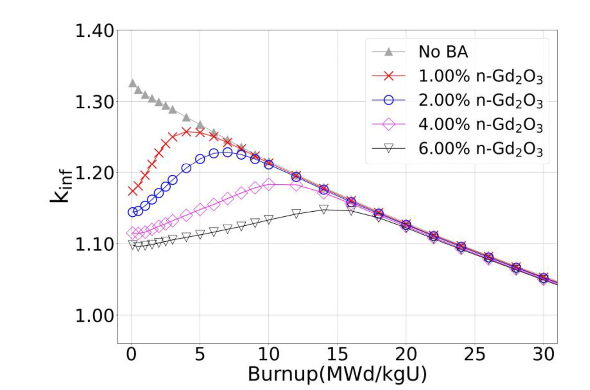
\includegraphics[width=0.78\linewidth]{images/lr_gd_kinf.pdf}
  \caption[Reactivity history of gadolinia-bearing fuel]{Multiplication factor against burnup for gadolinia contents of 1.00 to 6.00\,wt\%.\newline Figure taken from~\cite{gd_enriched_2021}.}
  \label{fig:lr-gd-kinf}
\end{figure}

In the submarine cores studied by Ippolito, this peak occurs where the
reactivity added by gadolinia depletion equals the reactivity lost to
uranium depletion~\cite{ippolito_1990}. A larger gadolinia content lowers
the peak and moves it to higher burnup~\cite{gd_enriched_2021}. After
burnout, the unburned poison and the fissile material it displaced leave a burnup penalty~\cite{alam_partI_2019}, which for natural gadolinia is small,
below $0.2\%\,\Delta k$ near 45\,GWd/MTU~\cite{ba_snf_2001}.

Gadolinia is also a means of limiting the soluble boron:

\begin{itemize}
  \item The U.S.\ EPR uses integral burnable absorbers in its first core,
        the initial fuel loading with which a new plant starts operation.
        With soluble boron alone, the moderator temperature coefficient of
        that core could be positive at the beginning of life, so the
        absorbers reduce the boron concentration and keep the coefficient
        negative at power~\cite{epr_fsar_ch4}.

  \item Low-concentration gadolinia rods combined with high-concentration
        ones lowered the boron concentration early in the cycle by up to
        300\,ppm, without loss of energy capability and without a peaking
        penalty~\cite{mildrum_segovia_2001}.

  \item Enriched gadolinia is the route taken by the i-SMR for
        soluble-boron-free operation~\cite{ismr_sbf_2024}.
\end{itemize}

Enriched gadolinium has also been studied for a Brazilian plant. For a
fuel assembly of Angra-2, the second nuclear power plant at Angra dos
Reis, Brazil, a parametric study enriched the $^{155}$Gd of a design with
only 1\,wt\% gadolinia. Above 40\,\% enrichment it suppressed the
reactivity better than the commercial design with 2\,wt\% gadolinia, and
its peak pin power stayed close to that design. The authors concluded
that enriched gadolinium is the more effective burnable absorber,
because a smaller gadolinia fraction is needed~\cite{angra2_gd_2018}.

The absorber finally moves the power peak. The rods that contain
gadolinia do not become the peak power rods, but the UO$_2$ rods of the
assemblies that carry them can~\cite{robinson_gd10}. Gadolinia rods
placed next to each other suppress their own power strongly, which
raises the power of the neighbouring UO$_2$ rods and the pin peaking
factor~\cite{radaideh_2021_rl}. Operating experience covers high
concentrations, with about 550 rods at 8\,wt\% and 32 rods at 10\,wt\%
gadolinia irradiated in pressurised water reactors by November
1986~\cite{robinson_gd10}.
